\begin{frame}
\frametitle{What do we talk about when we talk about Dirac?}
\begin{columns}
\column{0.35\textwidth}
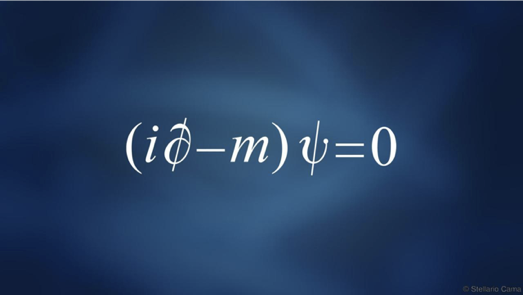
\includegraphics[scale=0.20]{dirac-eq.png}
 
 \column{0.6\textwidth}
%\begin{block}{}
If neutrinos were fermions of spin 1/2 they could presumably described by Dirac equation. Dirac had proposed his famous equation in 1928, two years before the neutrino was proposed by Pauli.  In 1929 P.A.M. Dirac had published his famous paper predicting antimatter (the positron), who would be discovered shortly after by Andersen. Yet, in 1930, antimatter was a concept as fantastic and hard to believe in as the neutrino itself.  

%\end{block}
\end{columns}
\end{frame}

\begin{frame}
\frametitle{The quantum theory of the electron}

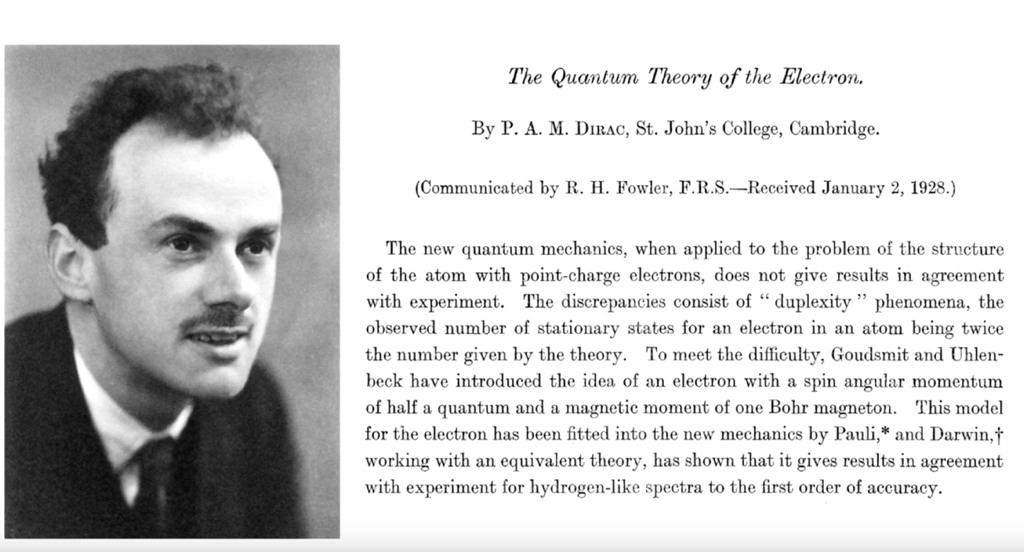
\includegraphics[scale=0.3]{dirac-eq-paper.png}
 
\end{frame}

\begin{frame}
\frametitle{The Klein Gordon equation}
The Dirac equation describes spin-1/2 particles such electrons and neutrinos. It emerges from Dirac's attempt to avoid the negative solutions in the equation of Klein-Gordon which is obtained when one quantizes the relativistic relation:
\[
E^2 = p^2 + m^2 \, \, {(\rm with~ c = 1)}
\]
through the quantum-mechanical recipe:
\[
E \rightarrow i \frac{\partial}{\partial_t}, \,\, \vv{\bm{P}} \rightarrow -i \vv{\bm{\nabla}}
\]
then we obtain the Klein Gordon equation


\begin{empheq}[box=\fbox]{align}
   (i \frac{\partial}{\partial_t})^2 \psi= [(-i \bar{\nabla})^2 + m^2] \psi \nonumber
\end{empheq}

%\[
%(i \frac{\partial}{\partial_t})^2 \psi= [(-i \bar{\nabla})^2 + m^2] \psi
%\]
%which is the KG equation. 

The wavefunction $\psi$~ is now a relativistic scalar and the space and time derivatives are both
second order. However, the initial values of $\psi$~  and
$\partial \psi$~  can be chosen freely, and as a result the probability density is no longer positive definite. 
This leaves open the possibility of negative probabilities.
\end{frame}

\begin{frame}
\frametitle{Linearizing $E = \sqrt{p^2 + m^2}$}
Dirac approach was to attempt linearizing the relativistic energy-momentum equation
\[
E = \sqrt{p^2 + m^2} = \vv{\bm{\alpha}}\cdot \vv{\bm{P}} + \beta \cdot m = 
\alpha_x p_x + \alpha_y p_y + \alpha_z p_z + \beta m
\]
Squaring both sides:

\begin{align*}
E^2 = p^2 + m^2 = & (\alpha_x p_x + \alpha_y p_y + \alpha_z p_z + \beta m) 
(\alpha_x p_x + \alpha_y p_y + \alpha_z p_z + \beta m) \\
%= & \alpha_x^2 p_x^2 + \alpha_y^2 p_y^2 + \alpha_z^2 p_z^2 + \beta^2 m^2 \\
%+ & (\alpha_x \alpha_y + \alpha_y \alpha_x) p_x p_y \\
%+ & (\alpha_x \alpha_z + \alpha_z \alpha_x) p_x p_z \\
%+ & (\alpha_y \alpha_z + \alpha_y \alpha_y) p_y p_z \\
%+ & (\alpha_x \beta + \beta \alpha_x) m p_x \\
%+ & (\alpha_y \beta + \beta \alpha_y) m p_y \\
%+ & (\alpha_z \beta + \beta \alpha_z) m p_z \\
= & p_x^2 + p_y^2 + p_z^2 + m^2
%
\end{align*}
The above equation can only be solved if the $\alpha_i, \beta$~are matrices of at least rank 4, which satisfy:
 \begin{empheq}[box=\fbox]{align}
  \{\alpha_i, \alpha_j\}&=0 \, \, ( i \neq j)\\ 
\{\alpha_i, \beta\} & = 0 \nonumber
\end{empheq}
where:
\[
\{A, B\} = AB + BA
\]
\end{frame}

\begin{frame}
\frametitle{Constructing $\bf{\alpha}$~and $\bf{\beta}$~using Pauli matrices }
%\begin{block}{}
%Since the $\alpha, \beta$~do not commute, they cannot be numbers. \alert{They need to be matrices}. In fact, they are traceless hermitian ($A^\dagger = A$) matrices or rank greater or equal than four. 
%\end{block}

They $\alpha, \beta$ can be constructed in terms of the  Pauli matrices:
\[
\alpha_i = 
\begin{pmatrix} 
0 & \sigma_i \\
\sigma_i & 0 
\end{pmatrix} \, \, ,
\beta = 
\begin{pmatrix} 
I & 0 \\
0 & -I 
\end{pmatrix} 
\]

where $I$~is the $2 \times 2$~ identity matrix, and the Pauli matrices are:
\[
\sigma_1 = 
\begin{pmatrix} 
0 & 1 \\
1& 0 
\end{pmatrix} \, \, ,
\sigma_2 = 
\begin{pmatrix} 
0 & -i \\
i & 0 \\ 
\end{pmatrix} \, \, ,
\sigma_3 = 
\begin{pmatrix} 
1 & 0 \\
0 & -1 \\ 
\end{pmatrix}
\]

Pauli matrices exhibit clearly the properties of being hermitian and traceless,
$\sigma_i^\dagger = \sigma_i$, $Tr \sigma_i = 0$, and $\sigma_i^2 = I$. They satisfy the commutation relations: 
\begin{empheq}[box=\fbox]{align}
 %\begin{empheq}[box=\tcbhighmath]{align}
\{\sigma_i, \sigma_j\}&=2 \delta_{ij} \, \, ( i,j,k = 1, 2, 3)\\
[\sigma_i, \sigma_j] & = 2 i \epsilon_{ijk} \sigma_k \nonumber
\end{empheq}
\end{frame}
\begin{frame}

\frametitle{The Dirac equation }
using the linearized equation
\[
E  -\va{\alpha}\cdot \va{P} - \beta \cdot m = 0
\]
and substituting operators
\[
E \rightarrow i \frac{\partial}{\partial_t}, \,\, \va{P} \rightarrow -i \va{\nabla}
\]
One obtains the Dirac equation
\[
 i \frac{\partial}{\partial_t} \psi = [ \va{\alpha} (-i\va{\nabla}) + m] \psi
\]

Multiply now $\beta$~from the left and define  the gamma matrices:
\[
 \gamma^0 = \beta = \begin{pmatrix} 
I & 0 \\
0 & -I 
\end{pmatrix}  \,\,\, ,  \gamma^i = \beta \alpha_i = \begin{pmatrix} 
0 & \sigma_i \\
-\sigma_i & 0 
\end{pmatrix} 
\]
To obtain 
%
%\begin{empheq}[box=\fbox]{align}
%(E \gamma^0 -\va{p}\cdot \va{\gamma} -m ) \psi & = 0 \nonumber
%\end{empheq}
%\[
%[i(\gamma^0 \partial_0 + \gamma^i \partial_i) -m ] \psi  = 0
%\]
%or
 \begin{empheq}[box=\fbox]{align}
(i \gamma^\mu \partial_\mu -m ) \psi & = 0 \nonumber
\end{empheq}
%\end{frame}

The  $\gamma$~matrices are not unique. Any set that satisfy the anticommutation relations (Clifford algebra) can be used:
%
\begin{empheq}[box=\fbox]{align}
\{\gamma^\mu, \gamma^\nu\} = 2 g^{\mu\nu} \nonumber
\end{empheq}
\end{frame}

%\begin{frame}
%Alternatively, in terms of the energy and momentum operators:
%\begin{empheq}[box=\fbox]{align}
%(E \gamma^0 -\va{p}\cdot \va{\gamma} -m ) \psi & = 0 \nonumber
%\end{empheq}
%
%In this equation $\psi$~is the Dirac bispinor: 
%\[
%\psi = \mqty(\psi_1 \\ \psi_2 \\ \psi_3 \\ \psi_4) =  \mqty(\phi \\ \chi); \,\,\,
%\phi =  \mqty(\phi_1 \\ \phi_2), \,\,\, \chi =  \mqty(\chi_1 \\ \chi_2)
%\]
%The two spinors $\phi$~and $\chi$~represent the particle and the antiparticle; the two components of each of them represent the two states of the third component of the spin, $s_z = +1/2$~and
%$s_z = -1/2$.
%
%The four $\gamma$~matrices, found before, are not unique. Any set that satisfy the anticommutation relations (Clifford algebra) can be used:
%
%\begin{empheq}[box=\fbox]{align}
%\{\gamma^\mu, \gamma^\nu\} = 2 g^{\mu\nu} \nonumber
%\end{empheq}
%\end{frame}


